\documentclass[tikz,border=10pt]{standalone}
\usepackage[T1]{fontenc}
\usepackage{lmodern}
\usetikzlibrary{arrows.meta, positioning}

\definecolor{ink}{HTML}{334155}
\definecolor{inputbg}{HTML}{F8FAFC}
\definecolor{sharedbg}{HTML}{EFF6FF}
\definecolor{actorbg}{HTML}{EEF2FF}
\definecolor{criticbg}{HTML}{ECFDF5}
\definecolor{tokenbg}{HTML}{FFF7ED}
\definecolor{outputbg}{HTML}{FEFCE8}

\tikzset{
  box/.style={
    draw=ink,
    rounded corners=5pt,
    line width=0.8pt,
    align=left,
    inner sep=7pt,
    font=\sffamily\small
  },
  input/.style={box, fill=inputbg, align=center, text width=55mm},
  process/.style={box, fill=sharedbg, align=center, text width=48mm},
  actor/.style={box, fill=actorbg, align=center, text width=50mm},
  critic/.style={box, fill=criticbg, align=center, text width=50mm},
  token/.style={box, fill=tokenbg, align=center, text width=52mm},
  output/.style={box, fill=outputbg, align=center, minimum width=31mm},
  note/.style={box, fill=inputbg, text width=52mm, font=\sffamily\footnotesize},
  arrow/.style={-{Latex[length=2.5mm]}, line width=0.8pt, draw=ink}
}

\begin{document}
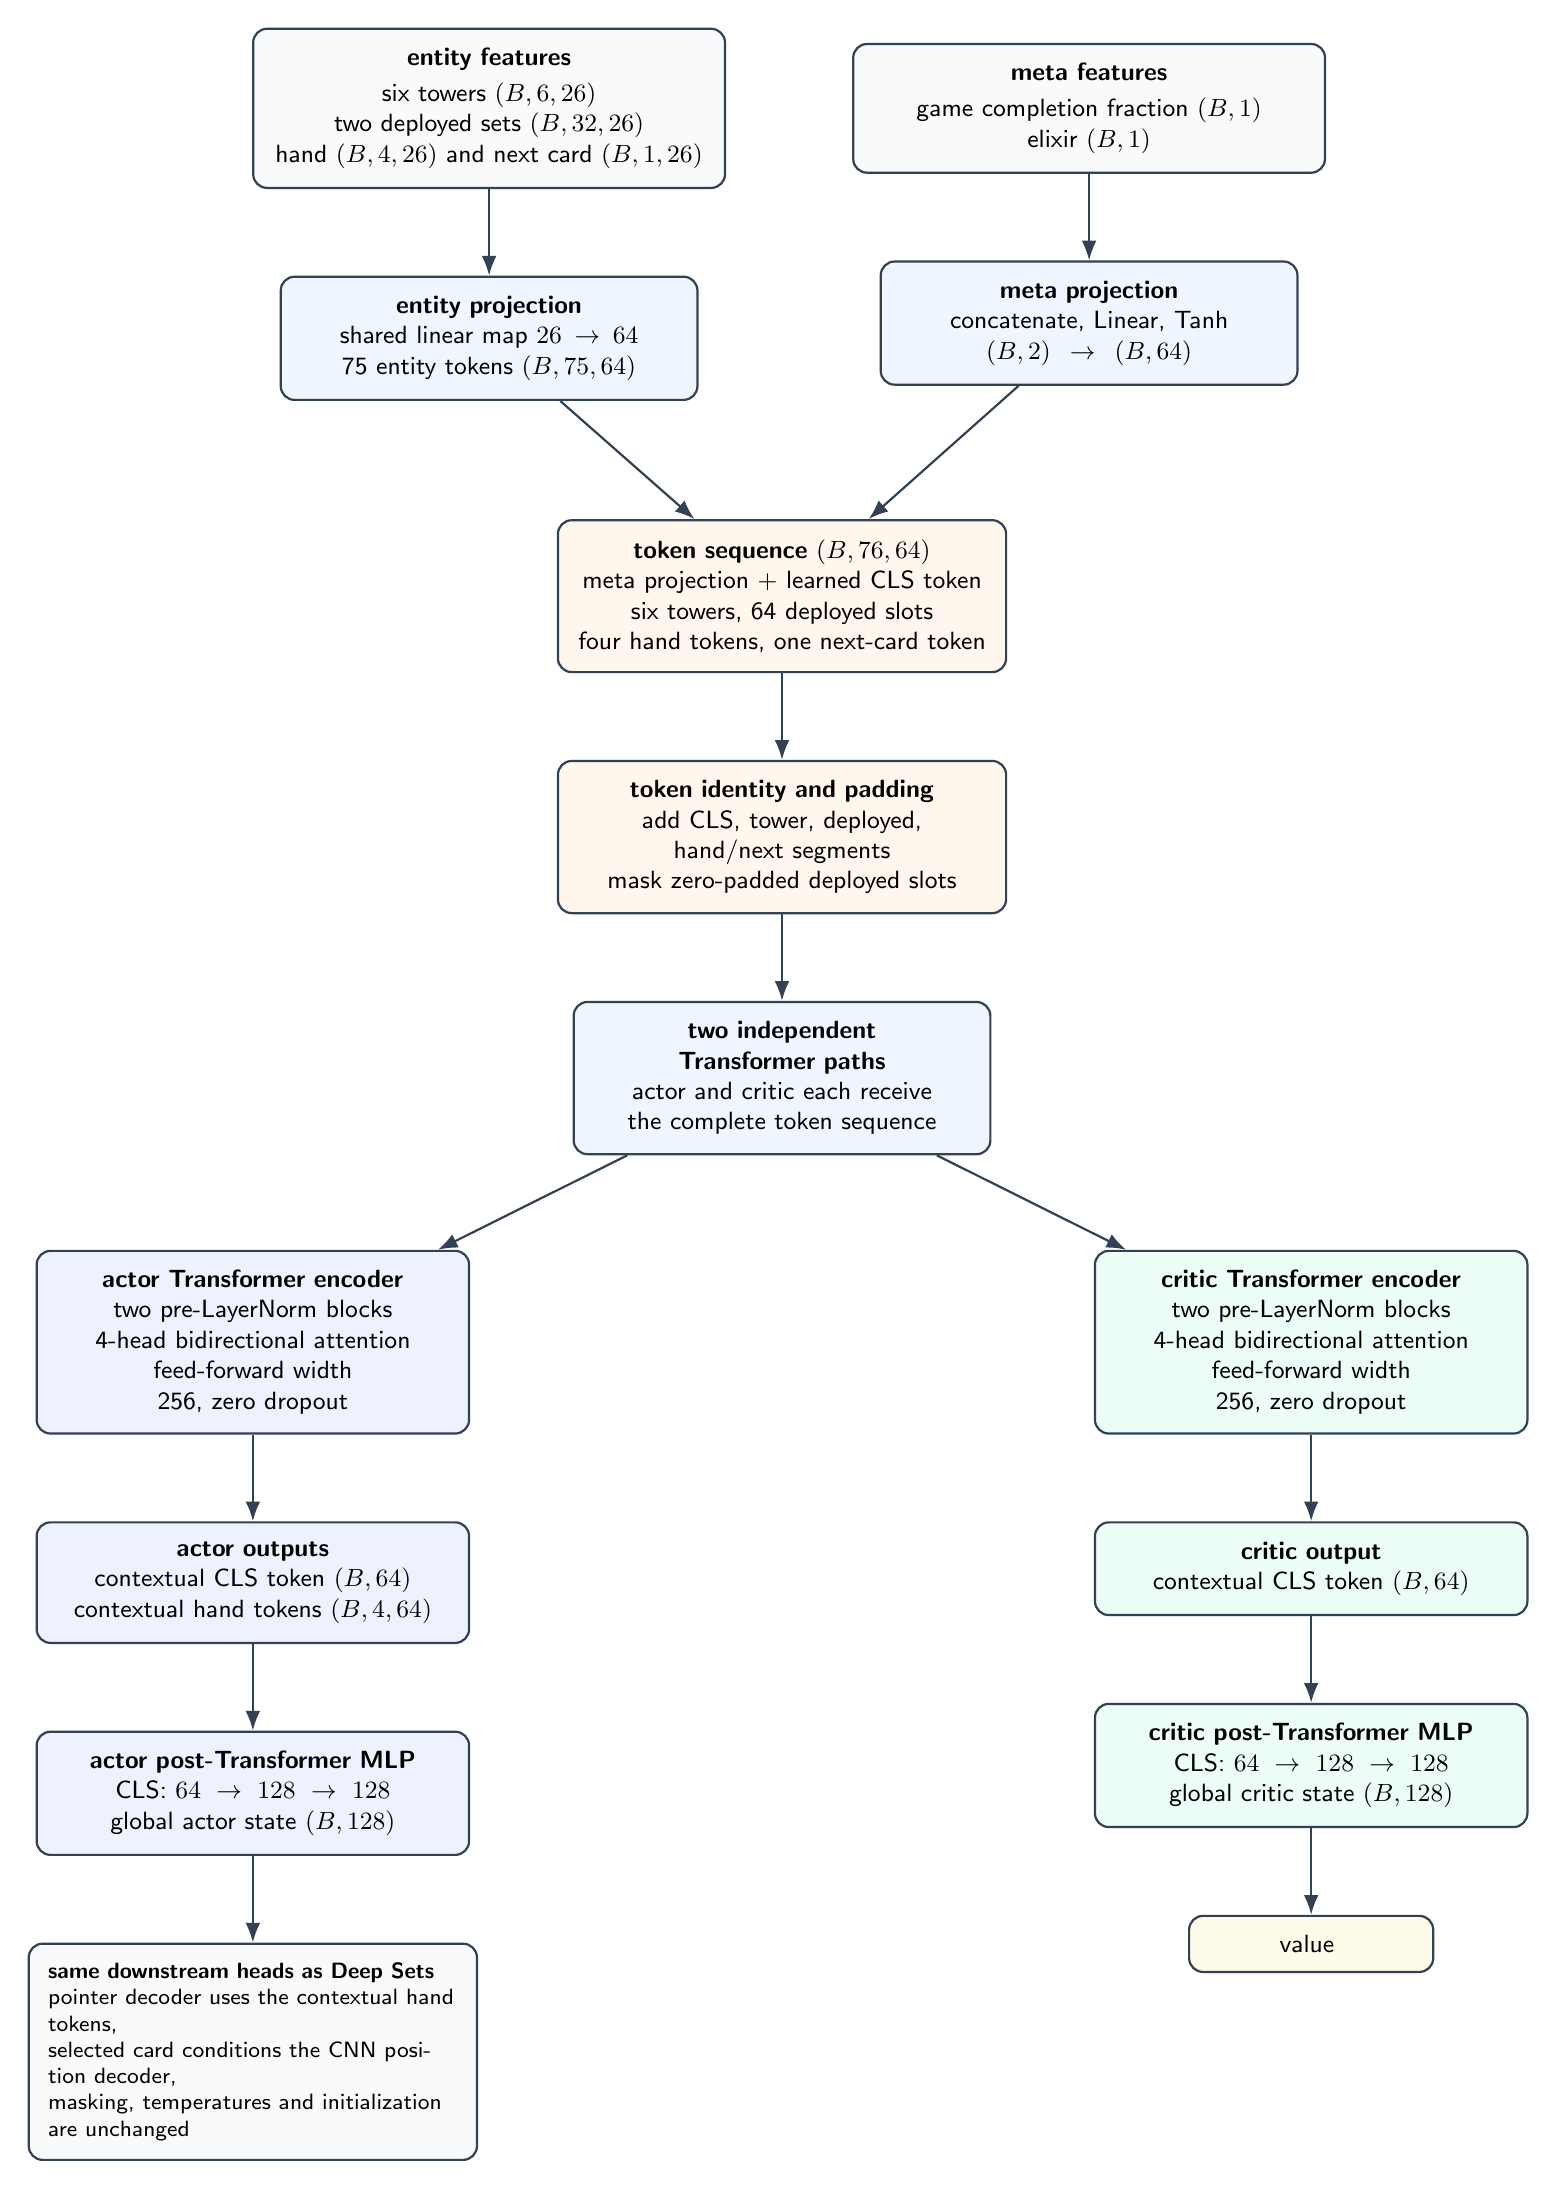
\begin{tikzpicture}[node distance=11mm and 16mm]

\node[input] (entities) {
  \textbf{entity features}\\[2pt]
  six towers $(B,6,26)$\\
  two deployed sets $(B,32,26)$\\
  hand $(B,4,26)$ and next card $(B,1,26)$
};

\node[input, right=of entities] (meta) {
  \textbf{meta features}\\[2pt]
  game completion fraction $(B,1)$\\
  elixir $(B,1)$
};

\node[process, below=of entities] (projection) {
  \textbf{entity projection}\\
  shared linear map $26\to64$\\
  75 entity tokens $(B,75,64)$
};

\node[process, below=of meta] (metaproj) {
  \textbf{meta projection}\\
  concatenate, Linear, Tanh\\
  $(B,2)\to(B,64)$
};

\node[token, below right=15mm and -18mm of projection] (sequence) {
  \textbf{token sequence $(B,76,64)$}\\
  meta projection + learned CLS token\\
  six towers, 64 deployed slots\\
  four hand tokens, one next-card token
};

\node[token, below=of sequence] (segments) {
  \textbf{token identity and padding}\\
  add CLS, tower, deployed, hand/next segments\\
  mask zero-padded deployed slots
};

\node[process, below=of segments] (split) {
  \textbf{two independent Transformer paths}\\
  actor and critic each receive\\
  the complete token sequence
};

\node[actor, below left=12mm and 13mm of split] (actorenc) {
  \textbf{actor Transformer encoder}\\
  two pre-LayerNorm blocks\\
  4-head bidirectional attention\\
  feed-forward width 256, zero dropout
};

\node[critic, below right=12mm and 13mm of split] (criticenc) {
  \textbf{critic Transformer encoder}\\
  two pre-LayerNorm blocks\\
  4-head bidirectional attention\\
  feed-forward width 256, zero dropout
};

\node[actor, below=of actorenc] (actorout) {
  \textbf{actor outputs}\\
  contextual CLS token $(B,64)$\\
  contextual hand tokens $(B,4,64)$
};

\node[critic, below=of criticenc] (criticout) {
  \textbf{critic output}\\
  contextual CLS token $(B,64)$
};

\node[actor, below=of actorout] (actorpost) {
  \textbf{actor post-Transformer MLP}\\
  CLS: $64\to128\to128$\\
  global actor state $(B,128)$
};

\node[critic, below=of criticout] (criticpost) {
  \textbf{critic post-Transformer MLP}\\
  CLS: $64\to128\to128$\\
  global critic state $(B,128)$
};

\node[output, below=of criticpost] (value) {
  value
};

\node[note, below=of actorpost] (sharedheads) {
  \textbf{same downstream heads as Deep Sets}\\
  pointer decoder uses the contextual hand tokens,\\
  selected card conditions the CNN position decoder,\\
  masking, temperatures and initialization are unchanged
};

\draw[arrow] (entities) -- (projection);
\draw[arrow] (meta) -- (metaproj);
\draw[arrow] (projection) -- (sequence);
\draw[arrow] (metaproj) -- (sequence);
\draw[arrow] (sequence) -- (segments);
\draw[arrow] (segments) -- (split);
\draw[arrow] (split) -- (actorenc);
\draw[arrow] (split) -- (criticenc);
\draw[arrow] (actorenc) -- (actorout);
\draw[arrow] (criticenc) -- (criticout);
\draw[arrow] (actorout) -- (actorpost);
\draw[arrow] (criticout) -- (criticpost);
\draw[arrow] (criticpost) -- (value);
\draw[arrow] (actorpost) -- (sharedheads);

\end{tikzpicture}
\end{document}
